
%\renewcommand{\Titulo}{\citetitle{MarcoNuno_CongArbIng_2014_07_00}}
\begin{frame}{\citetitle{MarcoNuno_CongArbIng_2014_07_00} (1)}
%\frametitle{\citetitle{\CitaF}}
%\note[item]{The next project in my presentation is called "Vehicle Tracking and Classification"· }
%\note[item]{We proposed a vision-based system to detect, track, count, and classify moving vehicles.}
\note[item]{Real-time vehicle tracking is crucial for traffic management systems, among other research areas.}
\note[item]{Each video has a duration of at least 90 seconds.  }
%
\note[item]{%The camera was mounted on a pedestrian footbridge over a main avenue, approximately 6.5 meters from the ground. 
This camera localization allows the system to have a wider view range for analyze vehicle's images }
%\note[item]{We published the presented results in the conference paper shown at the bottom of this slide. }

\begin{block}{Settings} 
\begin{columns}
\begin{column}{0.5\textwidth}
		\begin{itemize}
		%\item Four input videos of at least 90 seconds were captured and analyzed.
		\item We proposed a vision-based system to detect, track, count, and classify moving vehicles.
        \item We use a GoPro Hero 3 camera configured to 30 FPS rate. 
        \item The camera was mounted on a pedestrian footbridge over a main avenue, approximately 6.5 meters from the ground.
		\end{itemize}
\end{column}
\begin{column}{0.5\textwidth}  
    \begin{center}
     %%%%% this is a minipage, so \textwidth is already adjusted to the size of the column
     %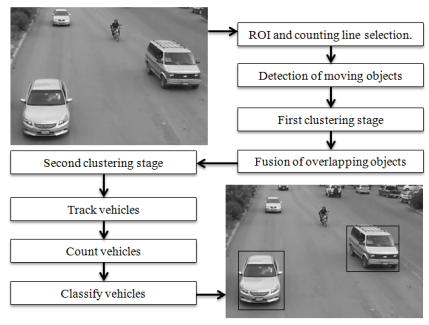
\includegraphics[width=0.8\textwidth]{Figs/TrafficFlow}
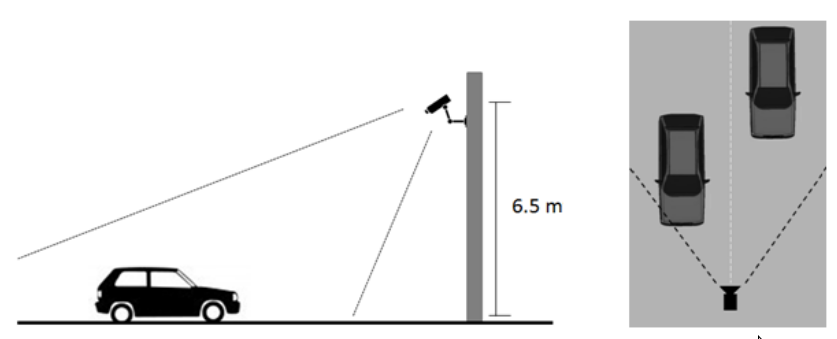
\includegraphics[width=1.0\textwidth]{Figs/VideosCapturadosParaControlVehicular}
     \end{center}
\end{column}
\end{columns}
\end{block} 

\footnotetext[1]{\fullcite{MarcoNuno_CongArbIng_2014_07_00}}
\setcounter{footnote}{0}
\end{frame}

\begin{frame}{\citetitle{MarcoNuno_CongArbIng_2014_07_00} (2)}
%\note[item]{The selection of a proper ROI size is crucial for the vehicle detection phase.}
\note[item]{To detect moving vehicles a temporal difference is applied. We obtained the pixel value difference between two consecutive frames, but the image is divided 
in n square segments with same length.}


\begin{block}{Blocks of the proposed system} 
\begin{columns}
\begin{column}{0.6\textwidth}
		\begin{enumerate}
\item The system is divided in several stages: ROI selection, detection of moving objects, clustering process, tracking, single-frame classification and counting. 	
        \item A (first) region clustering is performed to group the
different moving objects.
        \item A (second) region clustering is performed to estimate regions that belong to the same object (vehicle).
        \item A size, color and position analysis is performed to estimate the vehicle's type.
		\end{enumerate}
\end{column}
\begin{column}{0.4\textwidth}  
    \begin{center}
     %%%%% this is a minipage, so \textwidth is already adjusted to the size of the column
     \begin{tabular}{c}
         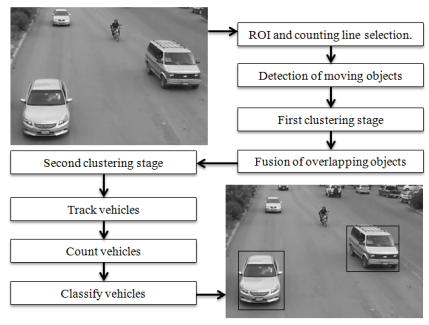
\includegraphics[width=0.7\textwidth]{Figs/TrafficFlow}\\
          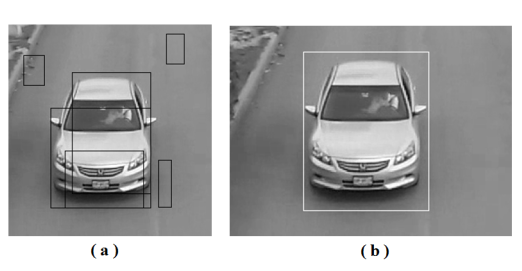
\includegraphics[width=0.5\textwidth]{Figs/RegionClustering_Vehicular}\\
      \end{tabular}
%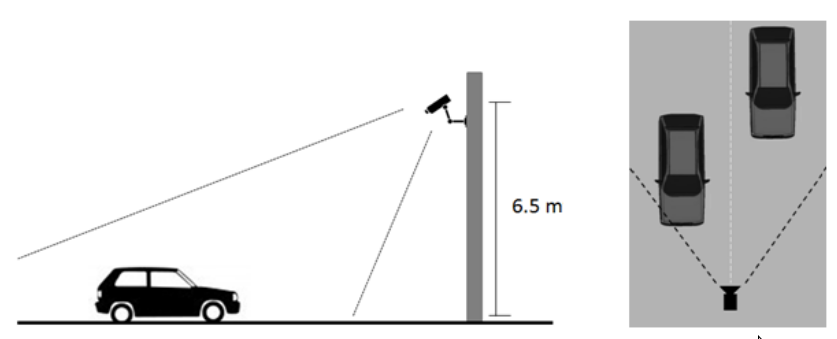
\includegraphics[width=0.8\textwidth]{Figs/VideosCapturadosParaControlVehicular}
     \end{center}
\end{column}
\end{columns}
\end{block} 



\end{frame}


\begin{frame}{\citetitle{MarcoNuno_CongArbIng_2014_07_00} (3)}

% S3
\note[item]{We create from the input videos a small dataset with 4 vehicle categories: small, compact, medium and large. The dataset has 164 samples, 4 for the small class, 128 for the compact class, 23 for the medium class and 4 for the large class.}
%\note[item]{The proposed algorithm performs better for high resolutions and small values of $K$}
\note[item]{The obtained results are related to the accuracy of vehicle classification method, using several sizes of $K$ for the grid, and testing for several resolutions (480p, 720p and 1080p). The higher resolution the higher accuracy but more the computational resources required to process the input video. }
\note[item]{In the left botton we show the classification and tracking results of selected frames of the input videos}
%\note[item]{The system does not work at night because the type of camera used.}
%\note[item]{Another improvement is to analyze each vehicle to detect some risk habits of drivers, such as texting or the absence of security bealt.}


\begin{block}{Results} 
\begin{columns}
\begin{column}{0.5\textwidth}
		\begin{itemize}
		\item Four classes of vehicles were considered: small, compact, medium and large.
		\item Cars dataset: 164 (total), 8 (small), 128 (compact), 23 (medium)
and 4 (large)
         \item Tested several video resolutions and grid sizes
		\item Improvements: 
		\begin{enumerate}
		\item Add an IR camera to support day and night illumination.
        \item Detect texting driver's among other risk situations.
        \end{enumerate}
		\end{itemize}
\end{column}
\begin{column}{0.5\textwidth}  
    \begin{center}
     %%%%% this is a minipage, so \textwidth is already adjusted to the size of the column
     \begin{tabular}{c}
    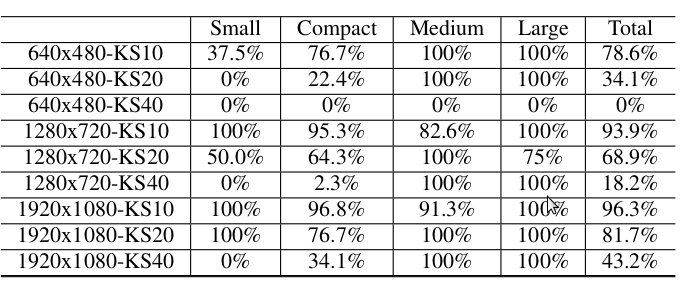
\includegraphics[width=0.8\textwidth]{Figs/VehicleClassificationResults}\\
    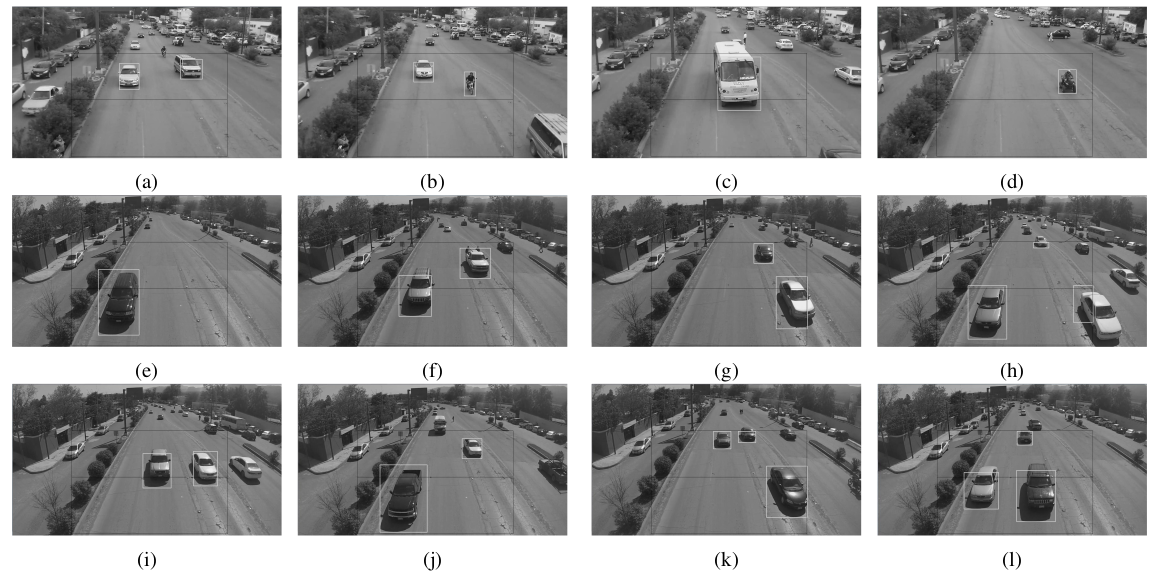
\includegraphics[width=0.8\textwidth]{Figs/TrafficFlow2}\\
               \end{tabular}
     \end{center}
\end{column}
\end{columns}
\end{block} 
\setcounter{footnote}{0}
\end{frame}

